\documentclass[border=10pt]{standalone}

\usepackage{tikz}
\usepackage{tikzsymbols}
\usetikzlibrary{calc,patterns,shapes.geometric}

\def\centerarc[#1](#2)(#3:#4:#5){\draw[#1] ($(#2)+({#5*cos(#3)},{#5*sin(#3)})$) arc (#3:#4:#5);}

\begin{document}
	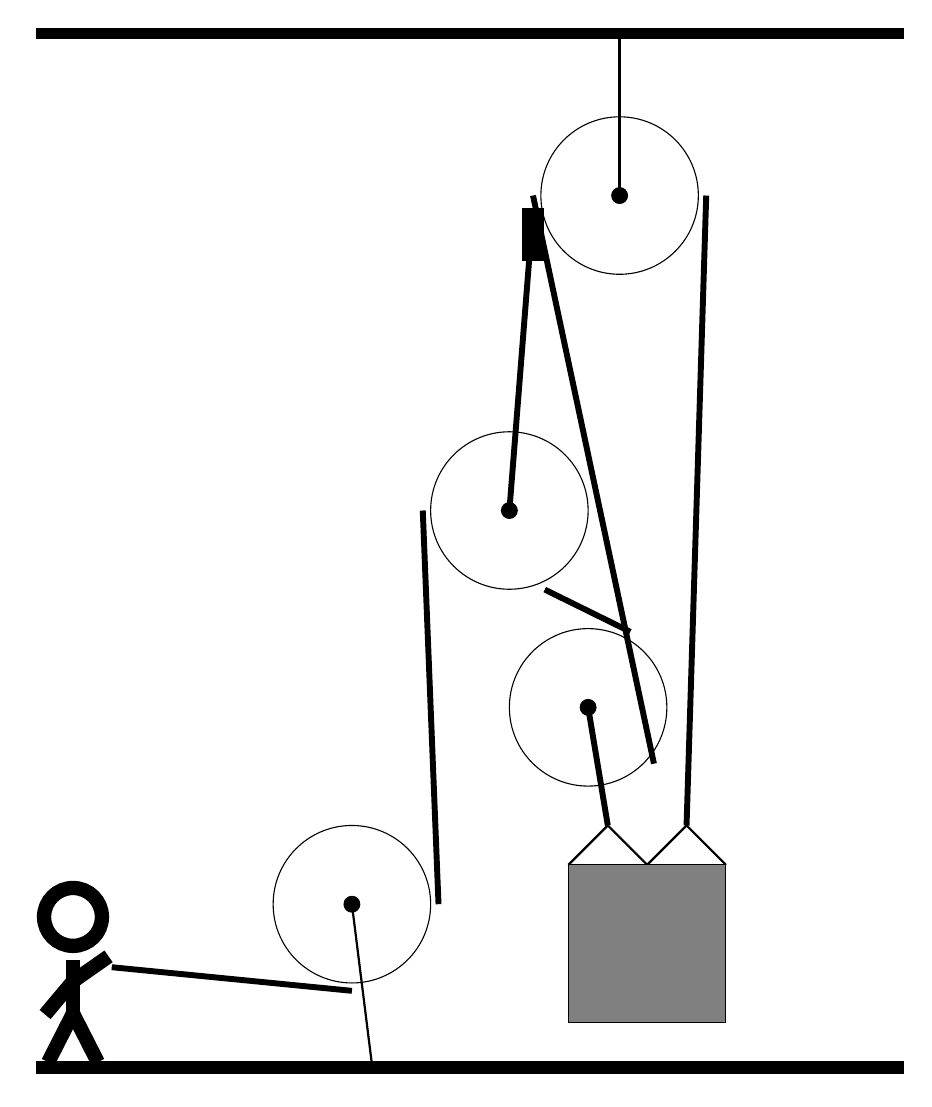
\begin{tikzpicture}
		%%%%% START %%%%%
		\draw[fill=black] (-6, 10) rectangle (5, 10.125);
		
		\draw (0, 4.0) circle (1);
		\draw[fill=black] (0, 4.0) circle (0.1);
		
		\draw (1, 1.5) circle (1);
		\draw[fill=black] (1, 1.5) circle (0.1);
		
		\draw (1.4, 8.0) circle (1);
		\draw[fill=black] (1.4, 8.0) circle (0.1);
		\draw[very thick] (1.4, 8.0) -- (1.4, 10);
		
		\draw (-2, -1.0) circle (1);
		\draw[fill=black] (-2, -1.0) circle (0.1);
		\draw[thick] (-2, -1.0) -- (-1.75, -3);
		
		
		\draw[thick]  (0.75, -0.5) -- (1.25, 0.0) -- (1.75, -0.5) -- (2.25, 0.0) -- (2.75, -0.5);
		\draw[fill=black!50] (0.75, -0.5) rectangle (2.75, -2.5);
		\draw[line width=0.75mm] (-5.05, -1.8) -- (-2, -2.1);
		\centerarc[line width=0.75mm](-2, -1.0)(270:360:1.1);
		\draw[line width=0.75mm] (-0.9, -1.0) -- (-1.1, 4.0);
		\draw[line width=0.75mm] (0, 4.0) -- (0.3, 7.8);
		\draw[line width=0.75mm, fill=black](0.2, 7.2) rectangle (0.4, 7.8);
		\centerarc[line width=0.75mm](0, 4.0)(-20:180:1.1);
		\draw[line width=0.75mm] (0.449, 2.996) -- (1.536, 2.46);
		\centerarc[line width=0.75mm](1, 1.5)(160:380:1.1);
		\draw[line width=0.75mm] (1.836, 0.785) -- (0.3, 8.0);
		\draw[line width=0.75mm](1, 1.5) -- (1.25, 0.0);
		\centerarc[line width=0.75mm](1.4, 8.0)(0:180:1.1);
		\draw[line width=0.75mm] (2.5, 8.0) -- (2.25, 0.0);
		
		\node at (-5.5, -1.9) {\Strichmaxerl[10][50][35]};
		
		\draw[fill=black] (-6, -3) rectangle (5, -3.15);
		%%%%% END %%%%%
	\end{tikzpicture}
\end{document}